\section{Basic Module}
Every Node (except the bridge node) consists of the same base module. It's
capable of measuring the ambient temperature and controlling four RGB-LEDs.
The functionality of the basic node can be extended by attaching another
module to the base module. 

There were multiple revisions of the basic node. Revision 1.0 was designed to
be a very rough prototype to test the functionality of the basic node and to 
test the concept of an attachable battery. Revision 2.0 was designed to be a 
more polished version of the basic node, all the other modules were designed 
and developed alongside this version.

The revisions of the basic node are presented backwards in this document, from
the latest to the oldest design.


\subsection{Hardware - V2.2}
\setAuthor{Richard Krammer}

    This section describes the latest hardware of the basic node. The basic node is a 
    simple node that can measure the ambient temperature and control four RGB-LEDs.
    The hardware consists of the following components:

    \begin{itemize}
        \item Microcontroller
        \item Temperature Sensor
        \item LED Indicator
        \item USB-C Connector
        \item 3.3V DC-DC Converter
        \item Module-Connector
    \end{itemize}
    \newpage

    \subsubsection{Microcontroller}
        The basic node uses an ESP32 C3 microcontroller. It is a low-power, highly
        integrated Wi-Fi and Bluetooth SoC. In the datasheet it was stated that the
        MCU is recommended for a wide range of applications, including smart home devices 
        and other IoT products.

        \begin{figure}[H]
            \centering
            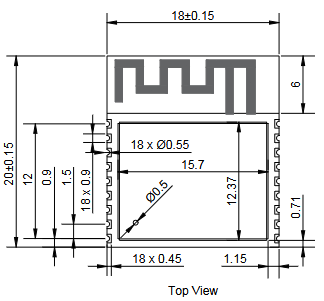
\includegraphics[height = 6cm]{assets/HW/ESP32-C3-sheet.png}
            \caption{ESP-C3 Datasheet in mm}
            
        \end{figure}

        It does not have as many GPIO pins compared to the ESP32-S3, however the abundance
        of GPIO pins is not necessary for the basic node. The ESP32 C3 is also cheaper and 
        alocates less space on the PCB.

        \begin{figure}[H]
            \centering
            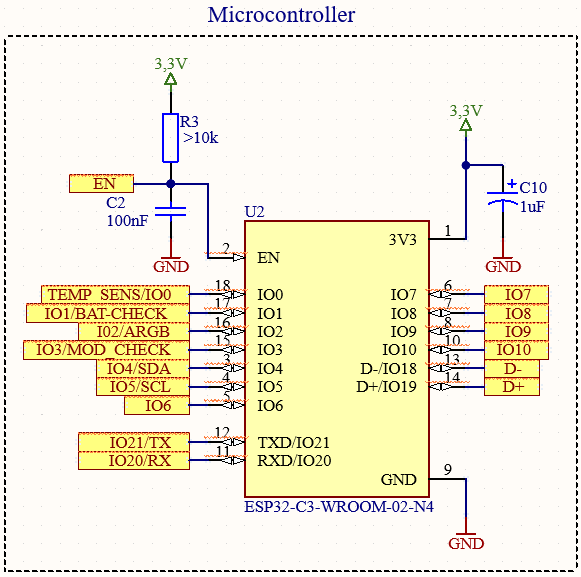
\includegraphics[height = 7.5cm]{assets/HW/ESP32-C3-schematic.png}
            \caption{ESP32-C3 implemented in the schematic.}
        \end{figure}


    \subsubsection{Temperature sensor}
        The DS18B20 was chosen as the temperature sensor. It is a digital thermometer
        with an operating temperature range of -55°C to +125°C. The sensor is connected
        to the microcontroller via GPIO0 and communicates over a 1-Wire bus.
        This sensor was used instead of the DHT11, for being smaller in size.

        \begin{figure}[H]
            \centering
            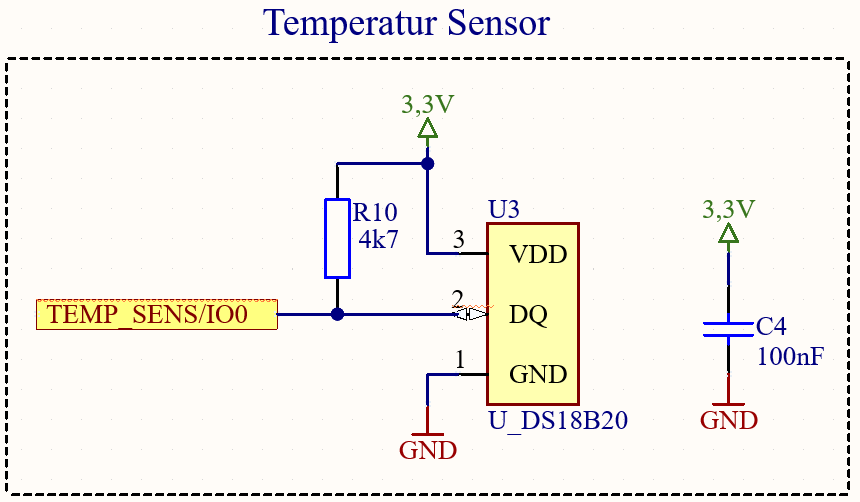
\includegraphics[width=0.7\textwidth]{assets/HW/DS18B20-schematic.png}
            \caption{DS18B20 implemented in the schematic.}
        \end{figure}

    \subsubsection{LED Indicator}
        The basic node has four WS2813b ARGB-LEDs. The LEDs are connected to the 
        microcontroller via GPIO 2. The LEDs are used to indicate the status of the node. 
        For example, the LEDs can be used to indicate the temperature range the node is in
        or to display the charge-level of the battery, when attached.

        \begin{figure}[H]
            \centering
            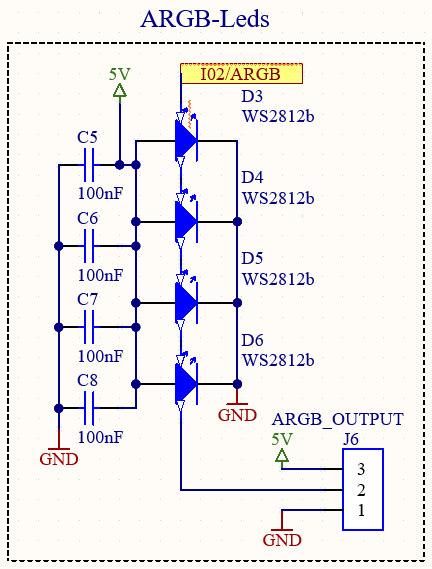
\includegraphics[width=0.4\textwidth]{assets/HW/RGB-LED-schematic.png}
            \caption{RGB-LEDs implemented in the schematic.}
        \end{figure}

    \subsubsection{USB-C Connector}

    The USB-C connector is used to power the basic node. This particular connector was
    chosen, duo to being the new standard for USB connectors, therefor being widely spread.
    
    \begin{figure}[H]
        \centering
        
\includegraphics[width=0.4\textwidth]{assets/HW/TBD2.png}
        \caption{USB-C Connector implemented in the schematic.}
    \end{figure}

    The USB protocol interacts with the charger to determine the power output. In order to
    power the basic node with 5V, a 5.1kOhm resistor is connected to the CC1 and CC2 pins.
    The resistor tells the charger that the basic node is a default USB device and can draw
    up to 3A of current. 
    \cite{noauthor_fugen_2023}
    
    \subsubsection{3.3V DC-DC Converter}

    The  step-down converter TLV62569 from Texas Instruments is used to convert 
    the 5V from the USB-C connector to 3.3V. The converter has a high efficiency
    of up to 95\%, which is significant for battery operation. It powers the
    microcontroller, temperature sensor and a module, if attached to the
    Module-Connector.

    \subsubsection{Module-Connector}

    The module connector is used to join additional modules to the basic module.
    The connector has 15 pins, 8 for power and powermanagment and 7 for 
    communication. 

    \begin{figure}[H]
        \centering
        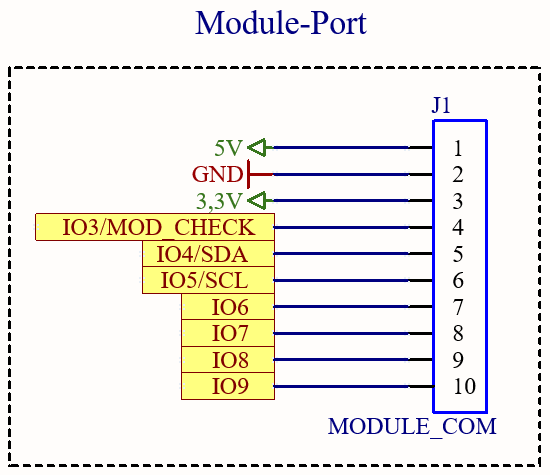
\includegraphics[width=0.4\textwidth]{assets/HW/Module-Connector-schematic.png}
        \caption{Module-Connector implemented in the schematic.}
    \end{figure}

    Pin 3-5 and 6-8 are symmetrical to each other. It was designed this way
    to allow the battery module and motion module to be attached simultaneously.
    The battery module is plugged into pin 1-5 and is connected to following 
    voltages:
    
    \begin{itemize}
        \item 1. VBAT - used to monitor the battery voltage
        \item 2. VBUS - used to charge and disable the battery module when the USB-C 
        is connected
        \item 3. 3V3 - not used, but may be relavant for future modules/revisions
        \item 4. GND
        \item 5. 5V - The battery module powers the basic node over this pin
    \end{itemize}

    Pin 6-15 are used for communication between the modules. 


    \subsubsection{Module-Detection}
    
    The basic node regonizes the attached module by measuring the voltage on pin 9.
    A 100kOhm resistor is installed on the base module pulling pin 9 to GND. 
    When a module is attached, a voltage devider is created. The voltage on pin 9 is 
    determinted by the second resistor on the module. The microcontroller reads the
    voltage and can determine the attached module. 
    
    \begin{figure}[H]
        \centering
        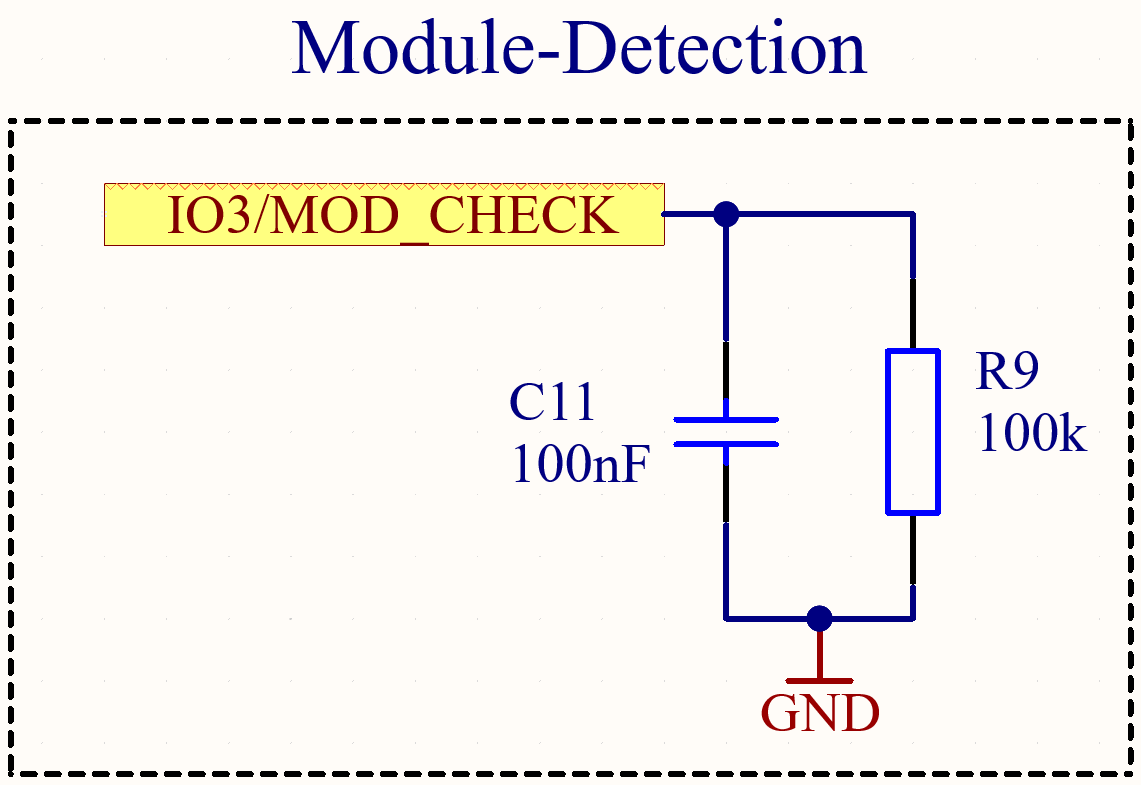
\includegraphics[width=0.4\textwidth]{assets/HW/Module-Detection-schematic.png}
        \caption{Module-Detection implemented on the base module.}
    \end{figure}

    \subsubsection{PCB}

    The PCB has a size of 30x75mm. The compenents used were mainly SMD components, 
    to keep the PCB small. 

    \begin{figure}[H]
        \centering
        
\includegraphics[width=0.7\textwidth]{assets/HW/TBD.png}
        \caption{PCB of the basic node. [Blue - Backside, Red - Frontside]}
    \end{figure}	


\subsection{Hardware - V2.1}

\subsection{Hardware - V2.0}

        
\subsection{Hardware - V1.1}
    Version 1.X of the basic module was inteeded to be a ruff prototype to test the concept of a 
    plugable battery powered module. For this reason only the battery module was designed for this
    version. Version 1.0 was never manifactured, but the design was used as a base for the
    version 1.1. The version 1.1 was manifactured and tested. 

    \subsubsection{Module-Connector}
        The module connector had three connectors, one for the battery and two for the
        module. The battery connector has a 5 pin header. 

        \begin{figure}[H]
            \centering
            
\includegraphics[width=0.6\textwidth]{assets/HW/TBD2.png}
            \caption{Module-Connector implemented in the schematic.}
        \end{figure}


        To connect a module there is a 10 pin header with IO-ports and a 6 pin header 
        for suppling power. It was not inteeded to design a module, besides the battery module,
        for this version. It was planned to be used in testing as an development board and connecting
        the sensors over jumper wires.

    \subsubsection{DC-DC Converter}
        
        To convert the 5V from the USB port to 3.3V a LM7805 linear regulator was used. This regulator
        would then be bybassed by the battery module when connected. Then the 3.3V would be supplied by the
        battery module. The 5V was also used to charge the battery.

        The LM7805 was turned off by a P-Channel MOSFET when the battery module was connected.

    \subsubsection{Seriel-To-USB Converter}
        The Seriel-To-USB converter was deamed to be unnassary since the MCU could also be programmed 
        over native USB, it was removed from later versions.

    \subsubsection{PCB}

\subsection{Hardware - V1.0}
\subsection{Base Software}
The base software is the foundation of every node. %NOT DONE AT ALL, THIS ALL WRONG

All slave nodes are customizable and modules can be swapped without flashing
the firmware. To implement this, module specific source code is executed in
its own thread. In the \texttt{Setup()} function, the module is determined
and the corresponding thread is started.

        \subsubsection{Determining the Module}

        \begin{figure}[H]
            \centering
            
\includegraphics[width=0.8\textwidth]{ThinkCorrectly.jpg}
            \caption{Node Module Selection}
            \label{fig:NodeModuleSelection}
        \end{figure}


